%
% skript.tex -- Lecture notes for the PartDiff lectures given at the
%               MSE Master
%
% (c) 2006-2018 Prof. Dr. Andreas Mueller, HSR
%
\documentclass[a4paper,12pt]{book}
\usepackage[utf8]{inputenc}
\usepackage[T1]{fontenc}
%\usepackage{german}
\usepackage{times}
\usepackage{csquotes}
\usepackage{multirow}
\usepackage{subfigure}
\usepackage{geometry}
\usepackage{csquotes}
\geometry{papersize={210mm,297mm},total={160mm,240mm},top=31mm,bindingoffset=15mm}
\usepackage{amsmath}
\usepackage{amssymb}
\usepackage{amsfonts}
\usepackage{amsthm}
\usepackage{amscd}
\usepackage{graphicx}
\usepackage{fancyhdr}
\usepackage{textcomp}
\usepackage{txfonts}
\usepackage[all]{xy}
\usepackage{paralist}
%\usepackage[colorlinks=true]{hyperref}
\usepackage[pdfborder={0 0 0}]{hyperref}
\usepackage{array}
\usepackage{tikz}
\usepackage{pdfpages}

%für Querformat von zeitplan
\usepackage{pdflscape}

%für Abbreviations
\usepackage{acronym}

%figure float
\usepackage{float}

%für python code
\usepackage{listings}

%bibliography
\usepackage[hyperref=true,backend=biber,style=ieee,defernumbers=true]{biblatex}
\addbibresource{references.bib}

%%%%%%%%%%%%%%%%%%%%%%%
%% Copyleft
%% Walter A. Kehowski
%% Department of Mathematics
%% Glendale Community College
%% walter.kehowski@gcmail.maricopa.edu
%% \begin{linsys}{2}
%% -x & + & 4y & = & 8\\
%% -3x & - & 2y & = & 6
%% \end{linsys}
%%%%%%%%%%%%%%%%%%%%%%%
%\makeatletter
%% math-mode column types ------------------
\newcolumntype{\linsysR}{>{$}r<{$}}
\newcolumntype{\linsysL}{>{$}l<{$}}
\newcolumntype{\linsysC}{>{$}c<{$}}
\newenvironment{linsys}[1]{%
\begin{tabular}{*{#1}{\linsysR@{\;}\linsysC}@{\;}\linsysR}}%
{\end{tabular}}
%\makeatother
\endinput

\makeindex


\begin{document}
\pagestyle{fancy}
\lhead{}
\rhead{}
\frontmatter
\newcommand\HRule{\noindent\rule{\linewidth}{1.5pt}}



\hypersetup{
	colorlinks=true,
	linktoc=all,
	linkcolor=blue
}


\newtheorem{satz}{Theorem}[chapter]
\newtheorem{problem}[satz]{Problem}
\newtheorem{hilfssatz}[satz]{Lemma}
\newtheorem{definition}[satz]{Definition}
\newtheorem{annahme}[satz]{Assumption}
\newtheorem{aufgabe}[satz]{Task}
\newenvironment{beispiel}[1][Example]{%
	\begin{proof}[#1]%
		\renewcommand{\qedsymbol}{$\bigcirc$}
	}{\end{proof}}
%\allowdisplaybreaks


\begin{titlepage}
\vspace*{\stretch{1}}
\HRule
\vspace*{10pt}
\begin{flushright}
{\LARGE
Fast Computer Vision based Geometry Estimation}

%\Large{with Rotation, GPS and On-Board-Diagnostics Sensor Data}
\end{flushright}
\begin{flushright}
{\Large Bachelor Thesis}
\end{flushright}
\HRule

\vspace{70pt}
\large
\textbf{Authors}

Cédric Renda, Manuel Tischhauser

\textbf{Supervisor}

Prof. Dr. Guido M. Schuster 

\textbf{Subject}

Image Processing



\vspace*{\stretch{2}}
\begin{center}
HSR Hochschule Für Technik Rapperswil

\today
\end{center}
\end{titlepage}


\chapter*{Abstract}

\section*{Introduction}
Mass production in the industry requires a periodical check of quality and dimensions of each part in different stations of the production chain.
In the special case of this thesis, the object to be measured is a steel spring.
Until today the spring has to be measured by hand by a production worker. In a production chain with a capacity of 200 springs per minute only some few springs actually get measured.
With conventional methods it s hard to get an accurate measurement because of the geometry of the spring and even harder to make these measurements reproducible because of the elasticity of the used steel.

This two difficulties can be solved by using cameras to estimate the geometry.
But such cameras and lenses suitable for such tasks are in many cases simply to expensive.

\section*{Approach}
It should be possible to compensate the flaws of a low-cost hardware by the software running on a platform with high computing power.
The software has to take into account and correct all the imperfections of the lens while at the same time manage to execute these task fast enough so the whole setup can be placed in the production chain.
Instead of making periodic measurements, it should this way be possible to estimate the geometry of every passing object.

In the case of the steel spring, the setup should be able to make accurate measurements (relative error = standard deviation/mean > 1\%).
With 200 springs per minute the setup has therefore to handle about 4 geometry estimations per second to be on the safe side.

Over the course of this thesis, a demonstrator, using a Raspberry Pi Camera Module V2, has been developed.
To demonstrate measurements performed on a moving object, the steel springs can be sidled over a tilted glass plate mounted in front of a backlight.
The camera is mounted parallel to the glass plate.
The software detects if a object moves through the field of view of the camera and measures the length and diameter.
These tasks are performed on a Nvidia Jetson Nano developer kit.

\section*{Conclusion}
In the static case, it was possible to achieve a relative error in the length of 0.22\% and in the diameter of 0.55\%.
With an object sliding with at an estimated speed of 2\,m/s over the glass plate, a relative error of 1.01\% in the length and 1.60\% in the diameter could be achieved.
The trigger checks for object in image with 21\,fps and the calculations can be performed at a rate of 15\,fps. 

\tableofcontents

\mainmatter

\chapter*{Abbreviations}
\addcontentsline{toc}{chapter}{Abbreviations} 
%A
\begin{acronym}
	\acro{rms}[RMS]{Root Mean Square}
\end{acronym}









\chapter{Introduction}
Production chains in the industry require a periodical measurement of the dimensions of the produced part.
If the measured values deviate to much from the desired value, the production has to be adjusted in order to keep the quality of the part.
In much cases this is done by a production worker who takes a random sample of produced parts and supervises this way the whole manufacturing process.

This thesis focuses on the manufacturing of steel springs.
Since the geometry of such a spring is rather complex, it is rather difficult to make a good measurement with conventional methods (e.g. manually).
Additionally, the elasticity of the steel makes it even more difficult to reproduce the measurements.

Estimating the geometry of the spring from the images taken by a camera mounted in the production chain could solve this problem, but optics used for measurements are usually too expensive.
Additionally, it would be very helpful to use multiple setups distributed over the whole production chain to determine in which production-step an error occurred.
This increases the cost for such a measurement device even more.
Since computing power is nowadays very cheap, these costs could be lowered dramatically by using a low-cost camera and compensating the cheap hardware with the software.

In this bachelor thesis, a device, called the demonstrator, has been developed to demonstrate the working principle of this setup.
In the first chapter the task analysis and approach will be evaluated.
The second chapter focuses on the general theory applied in the development.
The development itself will be described in more detail in Chapter three.
The fourth chapter discusses the results, followed by the conclusion in the sixth chapter. 

\newpage
\section{Task analysis}
The primary goal of this bachelor thesis was to develop a working demonstrator in order to show, that it really is feasible to make this kind of measurements with a low-cost device.
The demonstrator should be able to make measurements of length and diameter of the spring with a relative error (standard deviation/mean) of less than 1\%.
Since it is expected, that the production manufactures 200 springs per minute, the software which makes the necessary corrections an estimates the dimensions has to make about four measurements per second to be on the safe side.

\section{Approach}
It is reasonable to split this task into a hardware and a software part.

\subsection{Hardware}
The hardware consists of the following parts:
\begin{itemize}
	\item Raspberry Pi Camera Module V2
	\item Nvidia Jetson Nano developer kit
	\item Backlight illumination
	\item Mechanical construction
\end{itemize}
The Pi Camera Module delivers an image stream to the Jetson Nano where all the computing takes place.
To make the handling of the image easier, the spring is lit from the back with a specially designed illumination.
This makes it possible to threshold the incoming frames to a binary image, on which it is much easier (and faster) to operate on.
A mechanical construction consisting mainly of aluminum profiles serves as a framwork on which all other components can be attached.

\subsection{Software}
To compensate lens imperfections, the camera has to be calibrated and this has to be done for every camera once before using it.
The software later uses the results from the calibration to adjust the image.
A software trigger checks all the frames for the a passing object.
If it found such a frame it passes this image to the next section of the software which is responsible for following tasks:
\begin{itemize}
	\item Undistort the image using the results from the calibration
	\item Find a known pattern on the plane as reference
	\item Transform the image to correct a tilted view of the camera to the plane
	\item find the Object (spring) in the frame
	\item Estimate the geometry (length and diameter) of the object
\end{itemize} 


\chapter{Theory}\label{theory}
This chapter takes a closer look at the theory and technology applied in this thesis.

\section{Camera Calibration in OpenCV}
Camera calibration is needed to obtain camera parameters like focal length and center point.
Further, it provides a method to correct distortions caused by the imperfect optics according to a certain distortion models.
For that, a set of images of a known pattern (usually a checkerboard) have to be taken from different view-points an angles.
These points provide the training data which is needed to estimate all the coefficients.

This section describes the theory behind the calibration process in OpenCV 4.3.0, which is the latest version at the time of writing this thesis.
\subsection{The pinhole camera model}
The functions OpenCV provides to calibrate the camera use the so-called pinhole camera model \cite{cv_calib}.
This model describes, how a 3D-point specified in world-coordinates ($P_w$) is transformed to a 3D-point in camera-coordinates ($P_c$) and then further projected onto the image plane ($p$). After this step, the point is described as a 2D-point in pixel coordinates.  Figure \ref{theory:pin} illustrates this setup.
\begin{figure}[ht]
	\centering
	%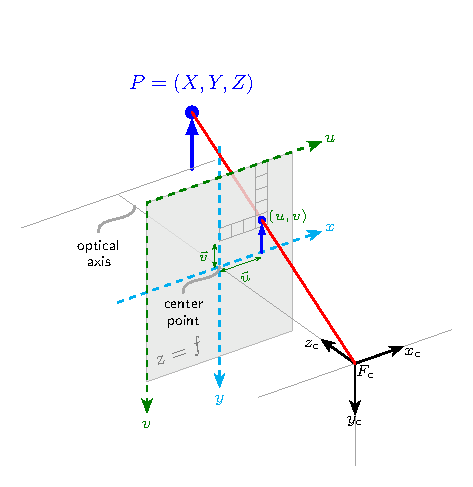
\includegraphics[width=0.9\textwidth]{2-theory/camera/camera.pdf}
	\caption{Pinhole-model (not up to date).\label{theory:pin}}
\end{figure} 

The transition from the world-coordinates to the camera-coordiantes can be described as 
\begin{align*}
\underbrace{\begin{pmatrix}
X_c\\
Y_c\\
Z_c\\
\end{pmatrix}}_{P_c}=
\underbrace{\begin{pmatrix}
r_{11}&r_{12}&r_{13}\\
r_{21}&r_{22}&r_{23}\\
r_{31}&r_{32}&r_{33}
\end{pmatrix}}_{R}
\underbrace{\begin{pmatrix}
X_w\\
Y_w\\
Z_w\\
\end{pmatrix}}_{P_w}+
\underbrace{\begin{pmatrix}
t_x\\
t_y\\
t_z\\
\end{pmatrix}}_{t}.
\end{align*}
The vector $P_w$ is first rotated by $R$ and the translated by $t$. This can be written in one single matrix:
\begin{align}
\begin{pmatrix}
X_c\\
Y_c\\
Z_c
\end{pmatrix}=
\begin{pmatrix}
r_{11}&r_{12}&r_{13}&t_x\\
r_{21}&r_{22}&r_{23}&t_y\\
r_{31}&r_{32}&r_{33}&t_z
\end{pmatrix}
\begin{pmatrix}
X_w\\
Y_w\\
Z_w\\
1
\end{pmatrix}\quad\Leftrightarrow\quad
P_c=
\begin{pmatrix}
R&|&t
\end{pmatrix}
\begin{pmatrix}
P_w\\
1
\end{pmatrix}\label{theory:world-camera}.
\end{align}

As a result of the theorem of intersecting lines, the projection from $P_c$ to $p$ is described as
\begin{align*}
\underbrace{\begin{pmatrix}
u\\
v
\end{pmatrix}}_{p}=
\begin{pmatrix}
f_x\cdot X_c/Z_c\\
f_y\cdot y_c/Z_c\\
\end{pmatrix}+
\begin{pmatrix}
c_x\\
c_y
\end{pmatrix}.
\end{align*}
where $f_x$ and $f_y$ are the focal length $f$ (in world units) normalized by their respective pixel size (in world units). Thus $f_x$ and $f_y$ are the same, if the pixels are quadratic.

By adding the principal point $\begin{pmatrix}c_x&c_y\end{pmatrix}^T$, which is usually close to the image center, it is taken into account, that pixel-coordinates are specified with respect to the upper left corner of the image plane. .
It is now simpler to write this in homogeneous coordinates:
\begin{align}
\begin{pmatrix}
u\\
v\\
1
\end{pmatrix}\sim s
\begin{pmatrix}
u\\
v\\
1
\end{pmatrix}=
\underbrace{\begin{pmatrix}
f_x&0&c_x\\
0&f_y&c_y\\
0&0&1
\end{pmatrix}}_{K}
\begin{pmatrix}
X_c\\
Y_c\\
Z_c
\end{pmatrix}\quad \Leftrightarrow \quad s
\begin{pmatrix}
p\\
1
\end{pmatrix}=
K\cdot P_c
\label{theory:camera-pixel},
\end{align}
where $s$ is an arbitrary scaling factor and $K$ is called the camera matrix.
The overall transition from world- to pixel-coordinates is the result of combining \ref{theory:world-camera} and \ref{theory:camera-pixel}:
\begin{align}
s
\begin{pmatrix}
u\\
v\\
1
\end{pmatrix}=
\begin{pmatrix}
f_x&0&c_x\\
0&f_y&c_y\\
0&0&1
\end{pmatrix}
\begin{pmatrix}
r_{11}&r_{12}&r_{13}&t_x\\
r_{21}&r_{22}&r_{23}&t_y\\
r_{31}&r_{32}&r_{33}&t_z
\end{pmatrix}
\begin{pmatrix}
X_w\\
Y_w\\
Z_w\\
1
\end{pmatrix}\quad \Leftrightarrow \quad s
\begin{pmatrix}
p\\
1
\end{pmatrix}=
K
\begin{pmatrix}
R&|&t
\end{pmatrix}
\begin{pmatrix}
P_w\\
1
\end{pmatrix}\label{theory:world-pixel}
\end{align}
The rotation and translation in $\begin{pmatrix}R&|&t\end{pmatrix}$ are called the extrinsic parameters. The camera matrix $K$ contains analogously the linear intrinsic parameters.

\subsection{The distortion model in OpenCV}
Non linear distortions, which appear before the projection in \ref{theory:camera-pixel} should be considered too.
OpenCV takes the effects of radial, tangential and thin prism distortion into account \cite{cv_calib}. 

\subsubsection{Radial Distortion}
Radial distortion is caused by the flawed curvature of the lens \cite{weng}.
It can be modeled with
\begin{align}
\begin{pmatrix}
x''\\
y''
\end{pmatrix}=
\begin{pmatrix}
x'\frac{1+k_1 r^2+k_2 r^4+k_3 r^6}{1+k_4 r^2+k_5r^4+k_6r^6}\\
y'\frac{1+k_1 r^2+k_2 r^4+k_3 r^6}{1+k_4 r^2+k_5r^4+k_6r^6}
\end{pmatrix}\label{theory:raddist},
\end{align}
where $x'$ and $y'$ are coordinates, described in camera-coordinates, normalized with $Z_c$
\begin{align*}
\begin{pmatrix}
x'\\
y'
\end{pmatrix}=
\begin{pmatrix}
X_c/Z_c\\
Y_c/Z_c
\end{pmatrix}
\end{align*}from
and r is the radius as taken with respect to the principal point $\begin{pmatrix}c_x&c_y\end{pmatrix}^T$
\begin{align*}
r^2 = x'^2 + y'^2.
\end{align*}
This type of distortion is symmetrical about the optical axis.
Figure \ref{theory:radial} illustrates the effect on a rectangle.
\begin{figure}[ht]
	\centering
	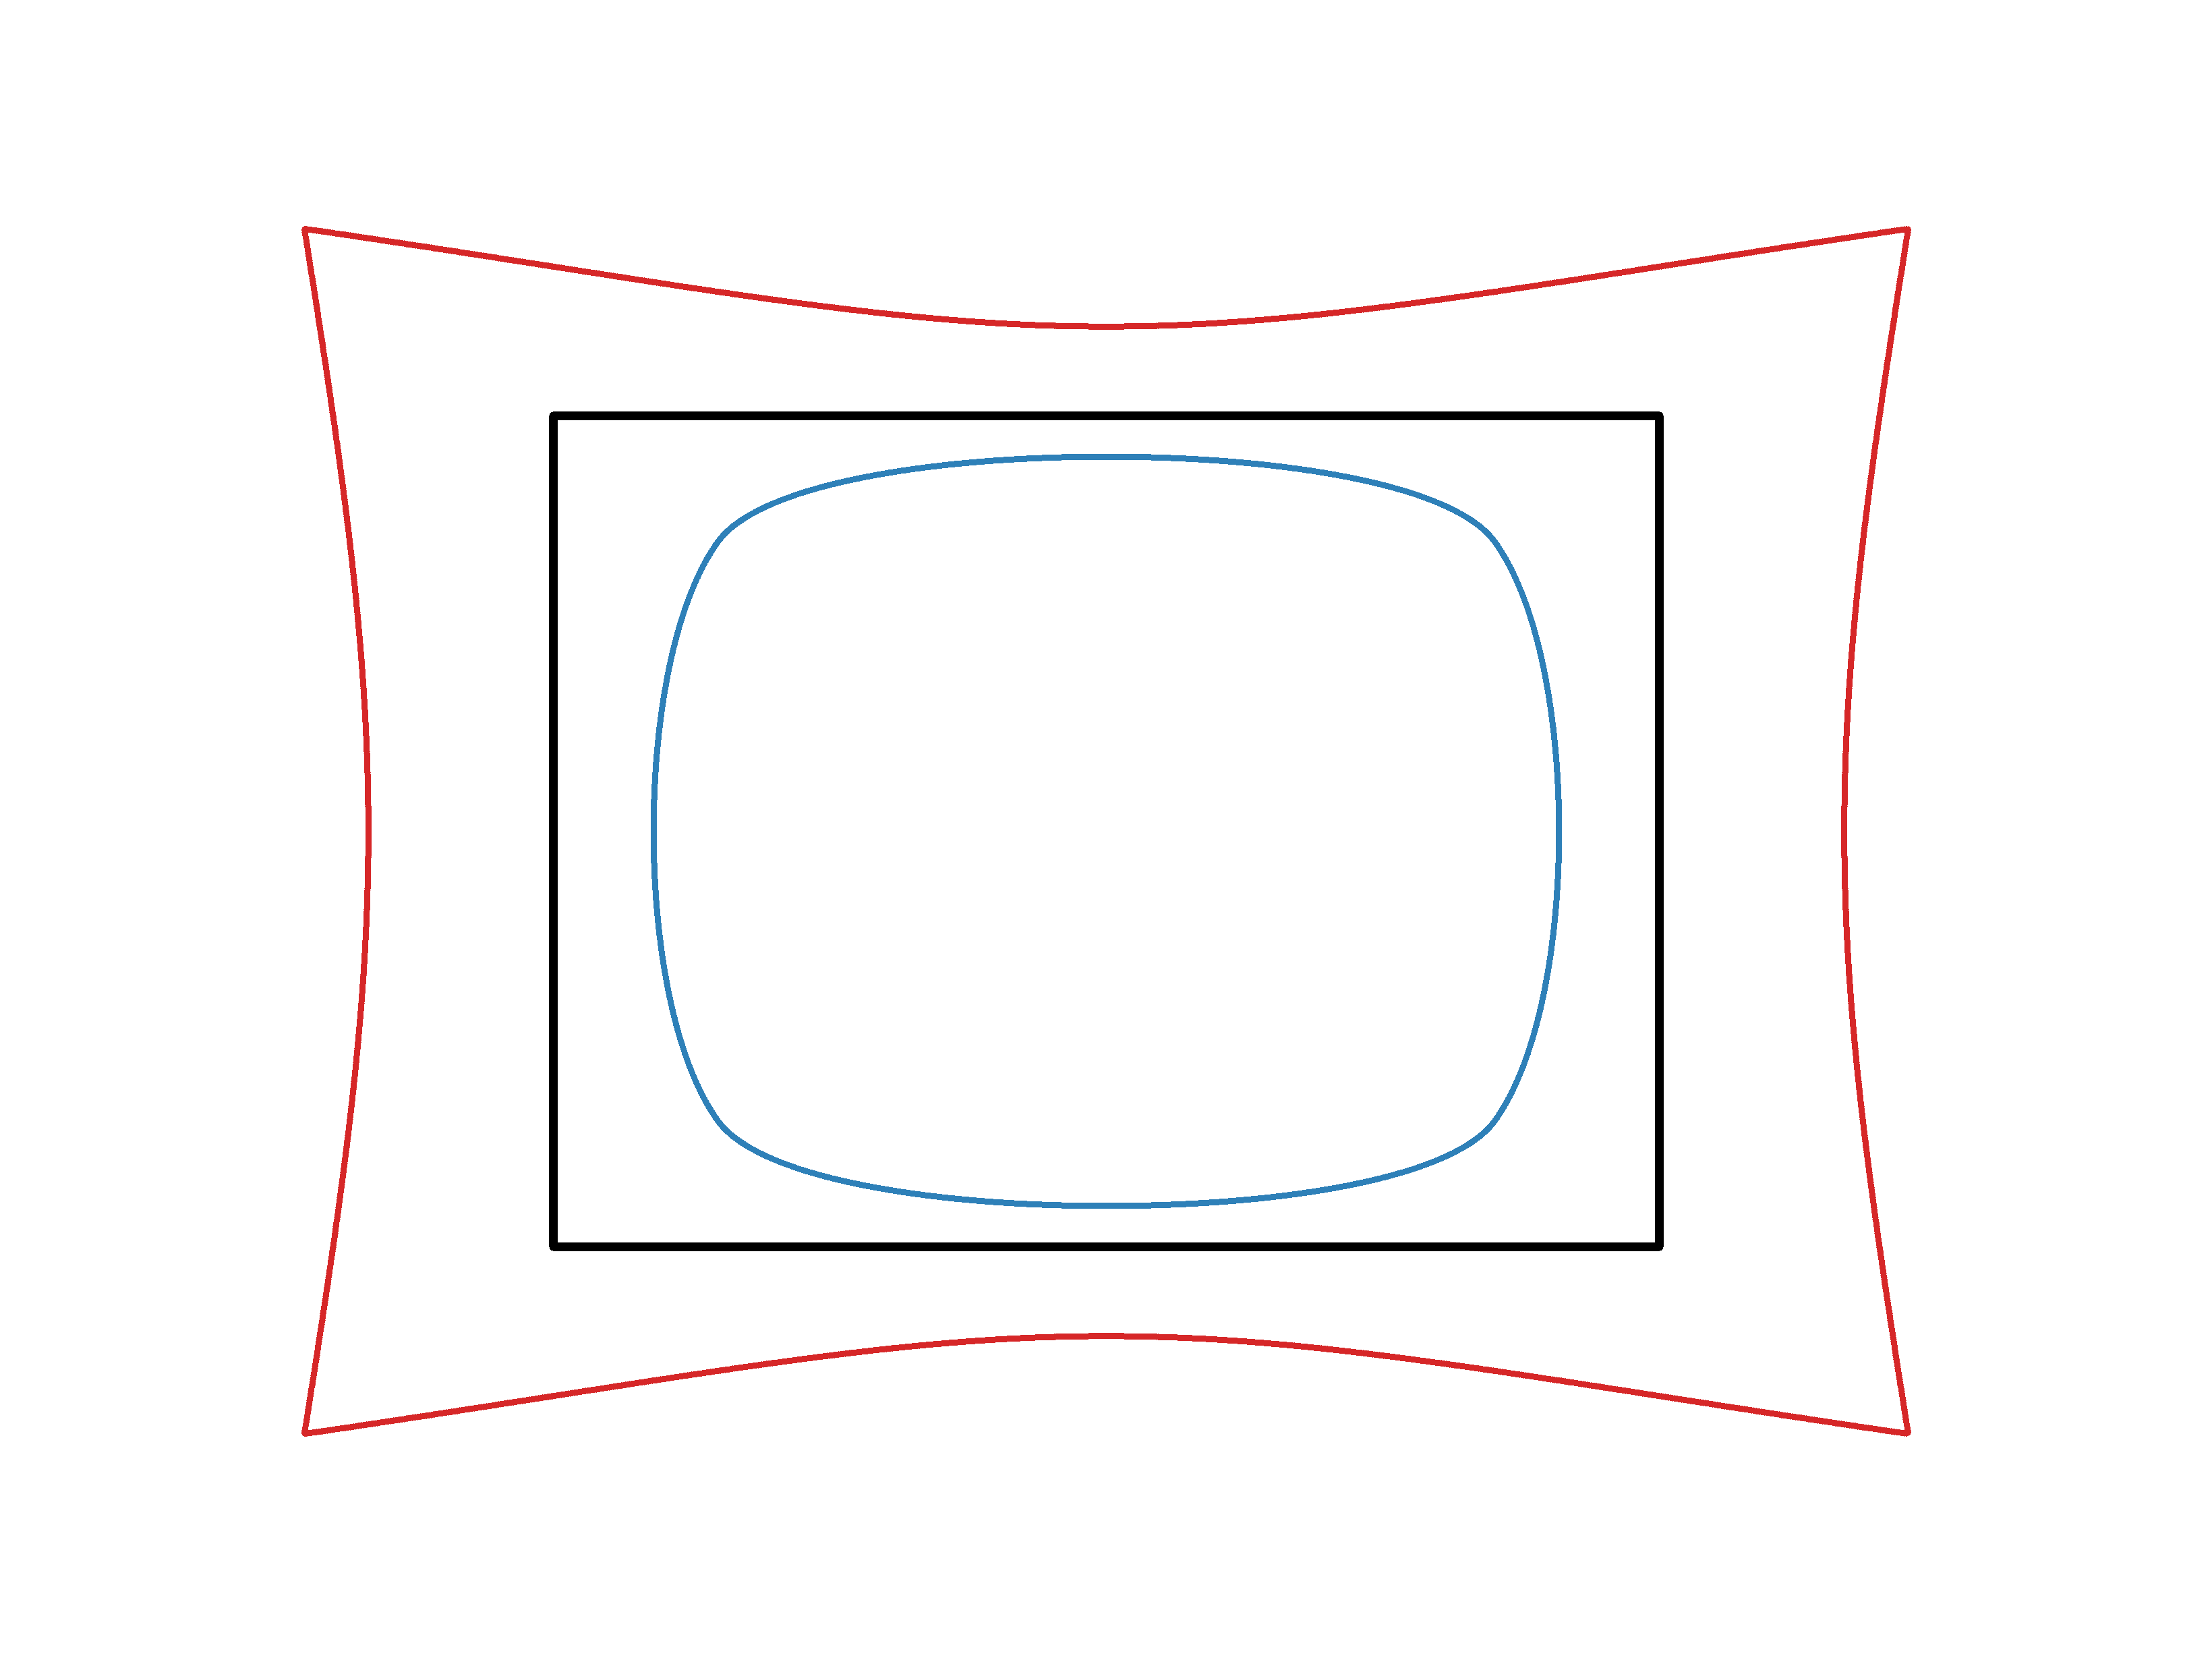
\includegraphics[width=0.9\textwidth]{2-theory/distortion/radial.png}
	\caption{Different types of radial distortion. Black: no distortion, red: $k_1 = 10$, $k_2=11$, $k_3=12$, $k_4=5$, $k_5=6$, $k_6=7$, blue: $k_1 = -2.2$, $k_2=-1.2$, $k_3=-0.8$, $k_4=-0.4$, $k_5=-0.3$, $k_6=-0.2$\label{theory:radial}}
\end{figure} 

\subsubsection{Tangential distortion}
Real optical systems are also subject to tangential distortion. This type of distortion has a decentering effect and occurs, if the line through the optical center of the lens and the principal point is not col-linear with the optical axis \cite{weng}.
The model
\begin{align}
\begin{pmatrix}
x''\\
y''
\end{pmatrix}=
\begin{pmatrix}
x' + 2p_1x'y'+p_2(r^2+2x'^2)\\
y' + 2p_2x'y'+p_1(r^2+2y'^2)
\end{pmatrix}\label{theory:tandist}
\end{align}
takes this into account.
Figure \ref{theory:tangential} shows the distortion this model introduces.

\begin{figure}[ht]
	\centering
	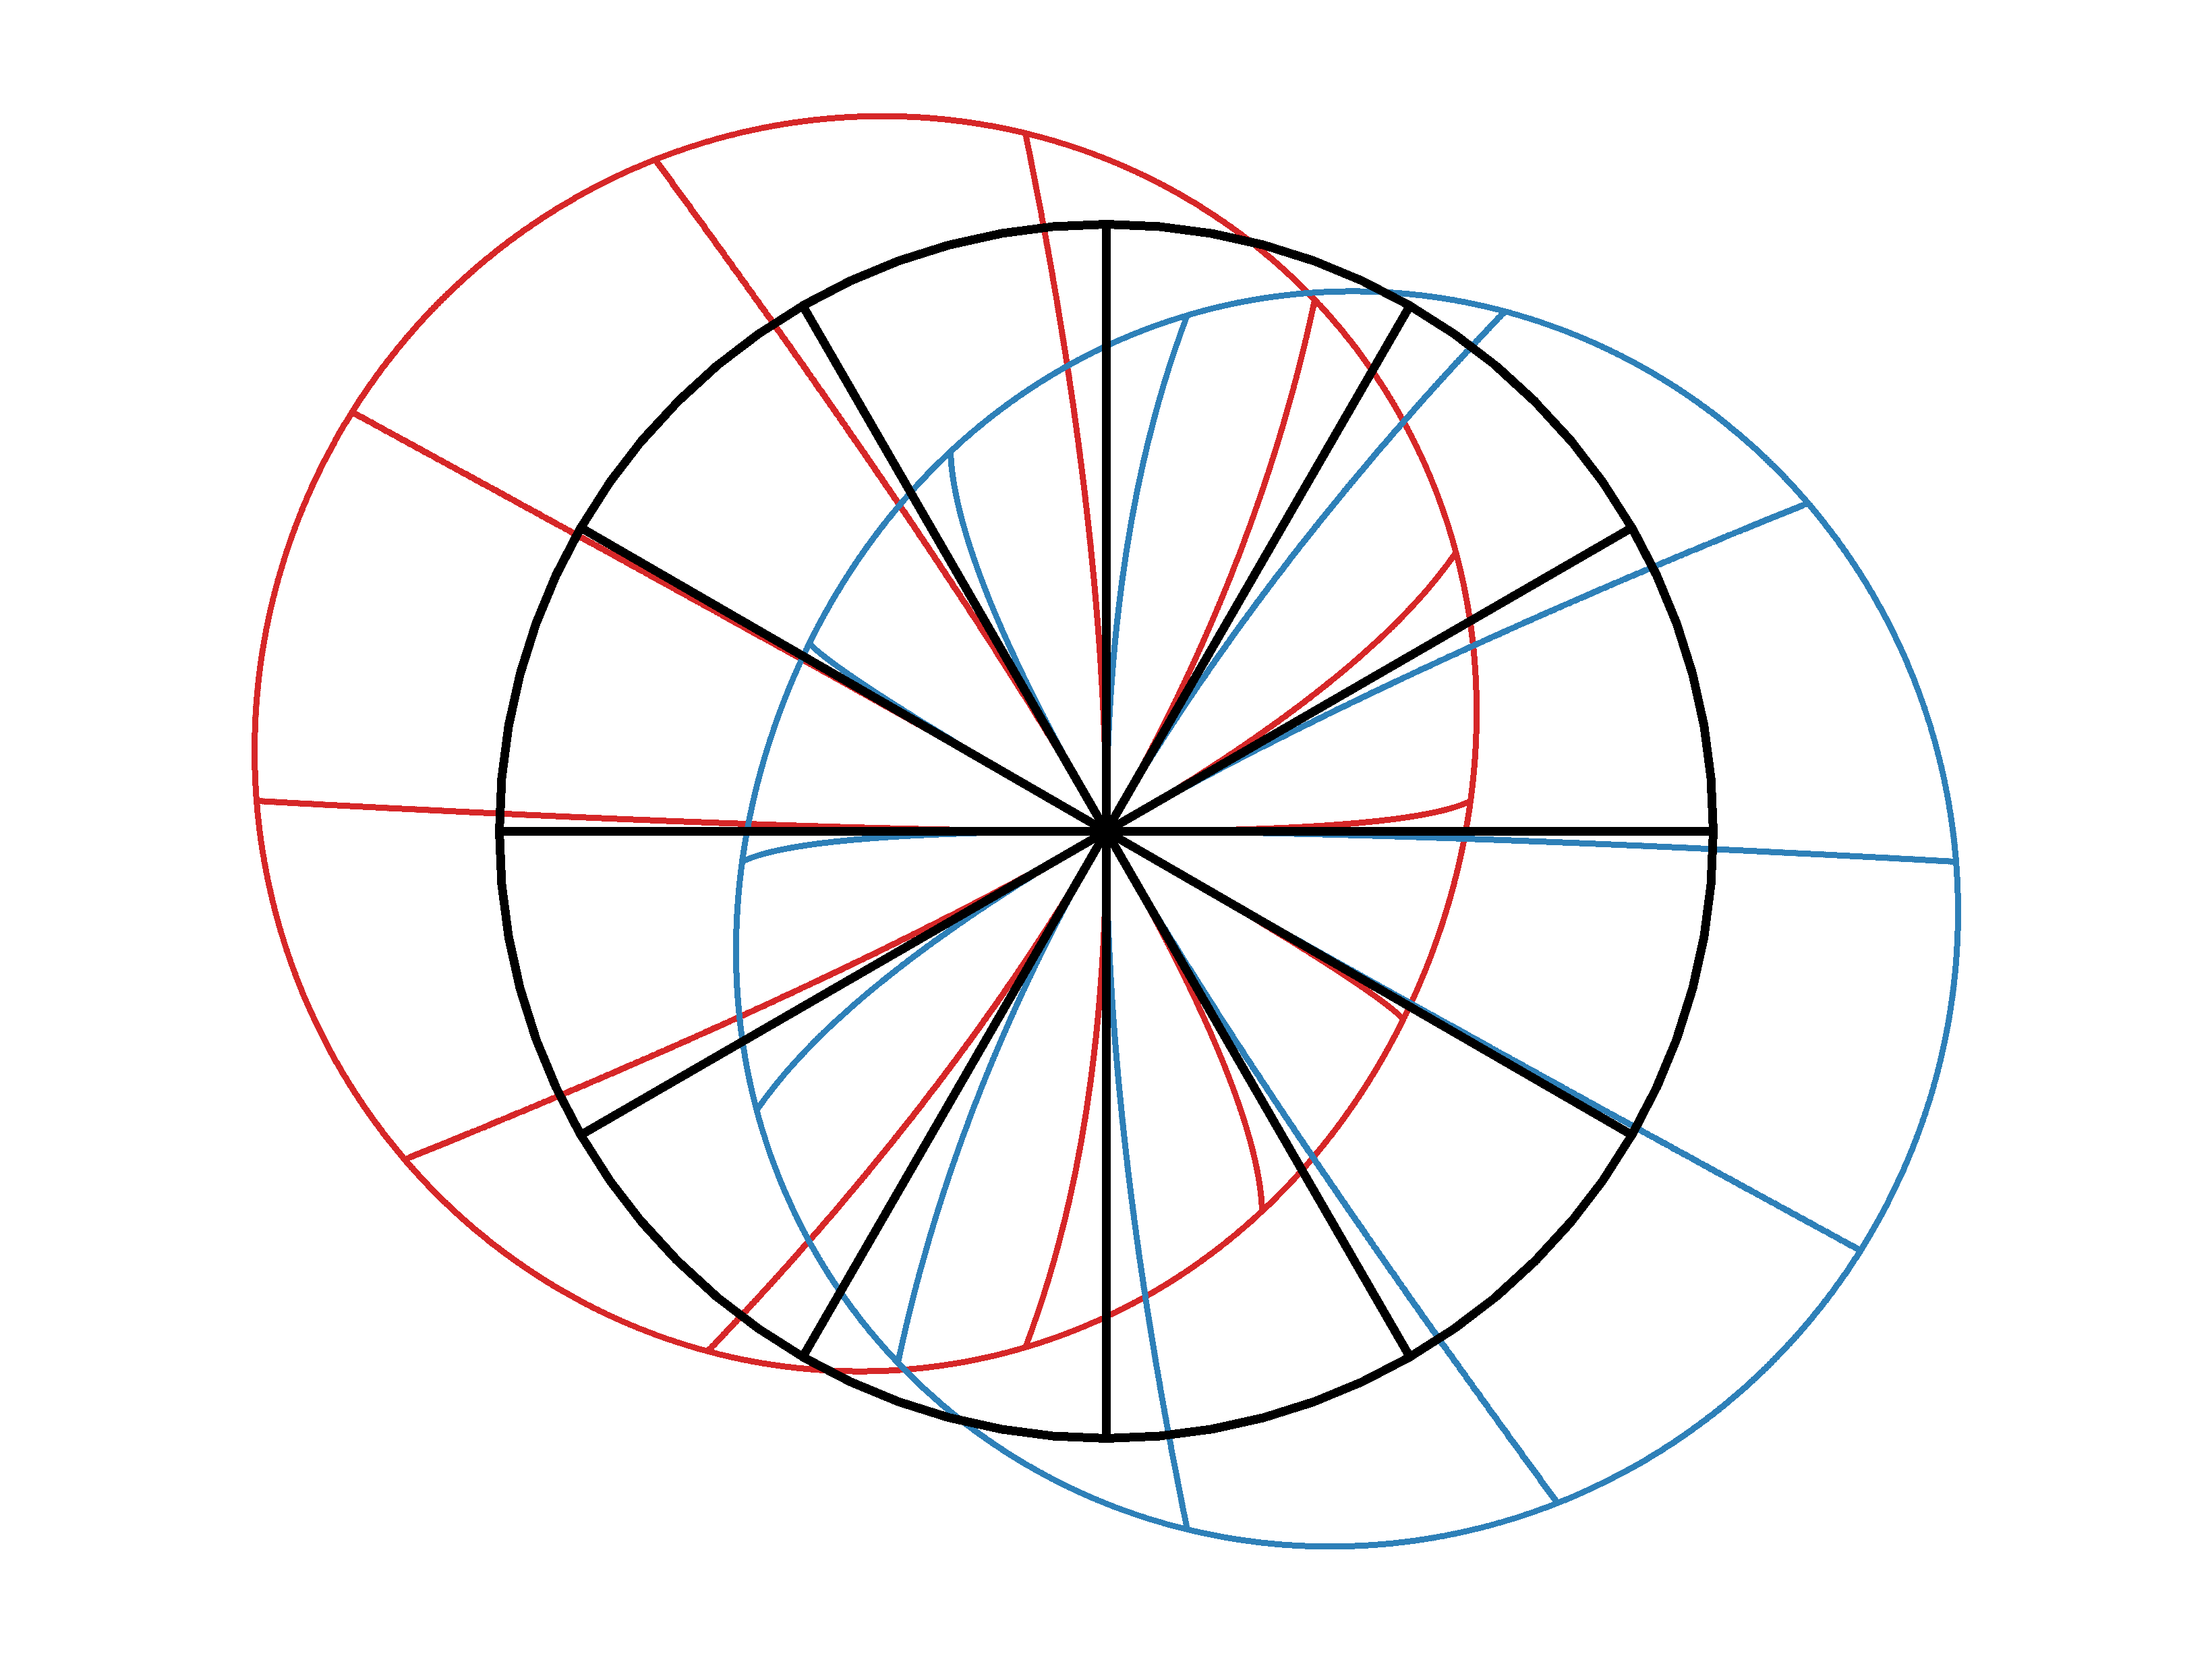
\includegraphics[width=0.9\textwidth]{2-theory/distortion/tangential.png}
	\caption{Different types of tangential distortion. Black: no distortion, red: $p_1 = -0.15$, $p_2=-0.4$, blue: $p_1 = 0.15$, $p2=-0.4$\label{theory:tangential}}
\end{figure} 

\subsubsection{Thin prism distortion}
Thin prism distortion is partially caused by lens imperfections and camera assembly \cite{weng}.
It introduces additional radial and tangential distortion, modeled with
\begin{align}
\begin{pmatrix}
x''\\
y''
\end{pmatrix}=
\begin{pmatrix}
x' + s_1 r^2 + s_2 r^4\\
y' + s_3 r^2 + s_4 r^4
\end{pmatrix}\label{theory:prismdist}.
\end{align}

\subsubsection{The combined model in OpenCV}
The models in \ref{theory:raddist}, \ref{theory:tandist} and \ref{theory:prismdist} combined result in
\begin{align}
\begin{pmatrix}
x''\\
y''
\end{pmatrix}=
\begin{pmatrix}
x'\frac{1+k_1 r^2+k_2 r^4+k_3 r^6}{1+k_4 r^2+k_5r^4+k_6r^6}+2p_1 x' y'+p_2(r^2+2x'^2)+s_1 r^2+s_2 r^4\\
y'\frac{1+k_1 r^2+k_2 r^4+k_3 r^6}{1+k_4 r^2+k_5r^4+k_6r^6}+2p_2x'y'+p_1(r^2+2y'^2)+s_3 r^2+s_4 r^4
\end{pmatrix}\label{theory:dist}.
\end{align}
In summary, a point in normalized camera-coordinates $\begin{pmatrix}x'&y'\end{pmatrix}^T$ is distorted as modeled in \ref{theory:dist}, which leads to the point $\begin{pmatrix}x''&y''\end{pmatrix}^T$. To get the distorted pixel-coordinates (subscript $d$), the projection has to be applied
\begin{align*}
\begin{pmatrix}
u_d\\
v_d\\
\end{pmatrix}=
\begin{pmatrix}
x''f_x+c_x\\
y''f_y+c_y
\end{pmatrix}\quad\Leftrightarrow\quad
\begin{pmatrix}
u_d\\
v_d\\
1
\end{pmatrix}=K
\begin{pmatrix}
x''\\
y''\\
1
\end{pmatrix},
\end{align*}
which completes the model so far.
Keep in mind, that when correcting the distortion, equation \ref{theory:dist} has to be inverted.

\subsection{Reprojection error}
The reprojection error is a value to asses the quality of a calibration.
It is the error between the detected image point and the projection (using the obtained coefficients) of its corresponding world point onto the image plane.
Since it only uses the points, which where previously used to obtain the calibration-parameters, it can be interpreted as a training error rate.

Calibration functions in OpenCV return the overall \acs{rms} reprojection error \cite{cv_calib}.

\subsection{Error propagation as further quality assessment}
As argued before, the reprojection error is a training error rate.
A low reprojection error is therefore not necessarily enough to estimate, how good the calibration really performs.

OpenCV returns with its extended calibration functions not only the camera intrinsics, but also an estimated standard deviation of each coefficient \cite{cv_calib}.
Under assumption that low standard deviations suggest a good calibration, it is valid to combine all standard deviations into one value using the propagation of uncertainty.

The propagation of error states that influence of each error of the inputs $x_i$ on the output value $y$ of a function
\begin{align*}
	y = f(x_1, x_2,..,x_n)
\end{align*}
can be linearly approximated and summed up to:
\begin{align}
	\Delta y = \sqrt{\sum_{i=1}^{n}\left(\frac{\partial y}{\partial x_i}\Delta x_i \right)^2} \label{theory:prop}.
\end{align}

Applied to \ref{theory:dist}, this leads to
\begin{align*}
	\Delta x''=\sqrt{\sum_{i=1}^{6}\left(\frac{\partial x''}{\partial k_i}\Delta k_i \right)^2+\sum_{i=1}^{2}\left( \frac{\partial x''}{\partial p_i}\Delta p_i\right)^2+\sum_{i=1}^{4}\left( \frac{\partial x''}{\partial s_i}\Delta s_i\right)^2}
\end{align*}
and
\begin{align*}
	\Delta y''=\sqrt{\sum_{i=1}^{6}\left(\frac{\partial y''}{\partial k_i}\Delta k_i \right)^2+\sum_{i=1}^{2}\left( \frac{\partial y''}{\partial p_i}\Delta p_i\right)^2+\sum_{i=1}^{4}\left( \frac{\partial y''}{\partial s_i}\Delta s_i\right)^2}.
\end{align*}
It is at this point not intended to go into further computations of the derivatives.
If we look at pixel coordinates from the center of the image, btw. $c_x=0$ and $c_y=0$, the radius (distance from the centerpoint) can be expressed as
\begin{align*}
	r = \sqrt{(f_x\cdot x'')^2+(f_y\cdot y'')^2}
\end{align*}
and therefore, if errors in $f_x$ and $f_y$ are neglected, with the propagation in \ref{theory:prop} applied
\begin{align}
	\Delta r = \sqrt{\left(\frac{\partial r}{\partial x''} \Delta x''\right)^2+\left(\frac{\partial r}{\partial y''} \Delta y''\right)^2}\label{theory:delta_r}.
\end{align}
This value $\Delta r$ can now be plotted over half the diagonal of an image to compare calibration coefficients of different calibration approaches.



\section{Measurement with back-light illumination}
To measure the size and form of an object there are multiple ways. A popular way to get the contour is to place a light source behind the object desired to measure, and aim on the object with an camera. With this method the optical sensors get the silhouette of the object. 
\subsection{Short introduction to photometry}
Photometry is the science concerned with the electromagnetic radiation visible to the human eye. In this section some important basics used further in this paper are explained. The theories of the following sections were taken from the textbook Physik 2 \cite{ruh}
\subsubsection{Photometric quantities}
In principle the normal physical quantities and units such as watts and joules could be used for the measurements of light radiation. However, in order to take into account the spectral sensitivity of the human eye, special photometric quantities and units are introduced.\\

\begin{table}[ht]
\centering
\begin{tabular}{ |p{5cm} p{2cm}|p{5cm} p{2cm} p{2cm}|  }
	\hline
	\multicolumn{2}{|c}{Quantity}&\multicolumn{3}{|c|}{Unit} \\
	\hline\hline
	\multicolumn{1}{|c}{Name}			& \multicolumn{1}{|c|}{Symbol}	& \multicolumn{1}{c}{Name}	& \multicolumn{1}{|c|}{Symbol}	& \multicolumn{1}{|c|}{SI-unit}\\

	\hline
	Luminous flux		& \multicolumn{1}{|c|}{$\phi_v$}	& lumen		& \multicolumn{1}{|c|}{lm}& \multicolumn{1}{|c|}{W}\\
	Luminous intensity 	& \multicolumn{1}{|c|}{$I_v$} 		& candela	& \multicolumn{1}{|c|}{cd}& \multicolumn{1}{|c|}{W/sr}\\
	Luminance			& \multicolumn{1}{|c|}{$L_v$}		& candela/$\text{m}^2$	& \multicolumn{1}{|c|}{cd/$m^2$}& \multicolumn{1}{|c|}{W/$\text{m}^2$sr}\\
	Illuminace 			& \multicolumn{1}{|c|}{$E_v$} 		& lux (=lumen/$\text{m}^2$) 	& \multicolumn{1}{|c|}{lx}& \multicolumn{1}{|c|}{W/$\text{m}^2$}\\

	\hline
\end{tabular}
\end{table}


Luminous intensity or candela is the Luminous flux per unit solid angle. It describes the perceived power per unit solid angle. As example we assume to have a light with a 10 lumen strong light source. If the light beam is now focused into 1 steradian light beam, the beam would be 10 candela.\\
Luminace is used 
\begin{align*}
L_{\mathrm{v}}=\frac{\mathrm{d}^{2} \Phi_{\mathrm{v}}}{\mathrm{d} \Sigma \mathrm{d} \Omega_{\Sigma} \cos \theta_{\Sigma}}
\end{align*}


\subsubsection{Light source}
To model a light source it is assumed that the source is a very small point which emits the light rays in all directions and is measured in luminous flux. The density of the light rays is reduced with the factor $\frac{1}{r^2}$ with $r$ being the distance. Luminous intensity of the light is proportional to the density of the rays. This behavior has to do with the fact that the surface area $A$ of a sphere
\begin{align*}
A=\int_{0}^{2 \pi} \int_{0}^{\pi} r^{2} \sin \theta d \theta d \varphi=4 \pi r^{2}
\end{align*}
grows squared with the distance from the center $r$.
\begin{align*}
A = 4\pi r^2
\end{align*}
In photometry the usage of solid angle is very common.  
\begin{figure}[ht]
	\centering
	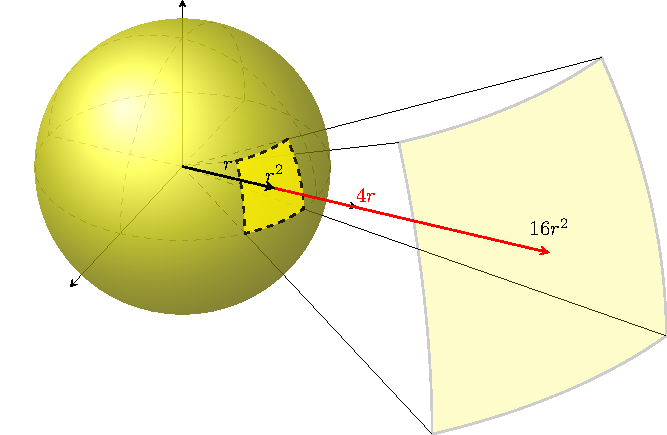
\includegraphics[width=0.6\textwidth]{2-theory/backlight/light.pdf}
	\caption{Light source in 3d\label{theory:light}}
\end{figure} 
\\

\subsubsection{Luminous flux}
Luminous flux or lumen is Luminous flux per unit time and has the unit candela steradians ($cd\cdot sr$). It is used to describe the total amount of light a lamp puts out. The 
\begin{table}[ht]
	\centering
	\begin{tabular}{ |p{5cm} p{2cm}|p{5cm} p{2cm} p{2cm}|  }
		\hline
		\multicolumn{2}{|c}{Quantity}&\multicolumn{3}{|c|}{Unit} \\
		\hline\hline
		\multicolumn{1}{|c}{Name}			& \multicolumn{1}{|c|}{Symbol}	& \multicolumn{1}{c}{Name}	& \multicolumn{1}{|c|}{Symbol}	& \multicolumn{1}{|c|}{SI-unit}\\
		
		\hline
		Luminous flux		& \multicolumn{1}{|c|}{$\phi_v$}	& lumen		& \multicolumn{1}{|c|}{lm}& \multicolumn{1}{|c|}{W}\\
		Luminous intensity 	& \multicolumn{1}{|c|}{$I_v$} 		& candela	& \multicolumn{1}{|c|}{cd}& \multicolumn{1}{|c|}{W/sr}\\
		Luminance			& \multicolumn{1}{|c|}{$L_v$}		& candela/$\text{m}^2$	& \multicolumn{1}{|c|}{cd/$m^2$}& \multicolumn{1}{|c|}{W/$\text{m}^2$sr}\\
		Illuminace 			& \multicolumn{1}{|c|}{$E_v$} 		& lux (=lumen/$\text{m}^2$) 	& \multicolumn{1}{|c|}{lx}& \multicolumn{1}{|c|}{W/$\text{m}^2$}\\
		
		\hline
	\end{tabular}
\end{table}


\lipsum[4]\\





\chapter{Evaluation}




\chapter{Development}
This chapter covers the developing process in more detail.



\chapter{Results}
This chapter covers the most important results.

\chapter{Conclusion}


%bibliography
\chapter*{References}
\addcontentsline{toc}{chapter}{References} 
\printbibliography[heading=none]

%Abbildungsverzeichnis
\addcontentsline{toc}{chapter}{List of figures} 
\listoffigures\thispagestyle{fancy}

%Tabellenverzeichnis
\addcontentsline{toc}{chapter}{List of tables} 
\listoftables\thispagestyle{fancy}

\addcontentsline{toc}{chapter}{Statement of Plagiarisms} 
\chapter*{Statement of Plagiarism}
%\textbf{Erkl�rung}\\
We declare that, apart from properly referenced quotations, this report is our
own work and contains no plagiarism; it has not been submitted previously
for any other assessed unit on this or other degree courses.
%Wir erkl�ren hiermit an Eides statt, dass ich die vorliegende Arbeit ohne Benutzung anderer als der angegebenen Hilfsmittel erstellt habe; die aus fremden Quellen direkt oder indirekt �bernommenen Gedanken sind als solche kenntlich gemacht. Die Arbeit wurde bisher in gleicher oder �hnlicher Form keiner anderen Pr�fungsbeh�rde vorgelegt und auch noch nicht ver�ffentlicht.\\
\vspace{0.8cm}\\

\begin{tabular}{l l}
    \textbf{Place} & \textbf{Date} \\
    Rapperswil  & \today
\end{tabular}
\vspace{0.8cm}

\textbf{Signatures}\\
\vspace{1.0cm}

Cedric Renda \hspace{3cm} Manuel Tischhauser

\clearpage



\appendix
\chapter{Partial derivatives of the distortion model\label{app}}
Shown are all partial derivatives of the distortion model in \ref{theory:dist} which are needed to implement the error propagation in subsection \ref{theory:error_propagation}.

\begin{align*}
\frac{\partial x''}{\partial k_1}&=\frac{r^2 x'}{1+k_4 r^2+k_5 r^4+k_6 r^6}&\frac{\partial x''}{\partial p_1}&=2x'y'\\
\frac{\partial x''}{\partial k_2}&=\frac{r^4 x'}{1+k_4 r^2+k_5 r^4+k_6 r^6}&\frac{\partial x''}{\partial p_2}&=r^2+2x'^2\\
\frac{\partial x''}{\partial k_3}&=\frac{r^6 x'}{1+k_4 r^2+k_5 r^4+k_6 r^6}&\frac{\partial x''}{\partial s_1}&=r^2\\
\frac{\partial x''}{\partial k_4}&=-r^2x'\frac{1+k_1 r^2+k_2 r^4+k_3 r^6}{(1+k_4 r^2+k_5 r^4+k_6 r^6)^2}&\frac{\partial x''}{\partial s_2}&=r^4\\
\frac{\partial x''}{\partial k_5}&=-r^4x'\frac{1+k_1 r^2+k_2 r^4+k_3 r^6}{(1+k_4 r^2+k_5 r^4+k_6 r^6)^2}&\frac{\partial x''}{\partial s_3}&=0\\
\frac{\partial x''}{\partial k_6}&=-r^6x'\frac{1+k_1 r^2+k_2 r^4+k_3 r^6}{(1+k_4 r^2+k_5 r^4+k_6 r^6)^2}&\frac{\partial x''}{\partial s_4}&=0\\
\end{align*}

\begin{align*}
\frac{\partial y''}{\partial k_1}&=\frac{r^2 x'}{1+k_4 r^2+k_5 r^4+k_6 r^6}&\frac{\partial y''}{\partial p_1}&=r^2+2y'^2\\
\frac{\partial y''}{\partial k_2}&=\frac{r^4 x'}{1+k_4 r^2+k_5 r^4+k_6 r^6}&\frac{\partial y''}{\partial p_2}&=2x'y'\\
\frac{\partial y''}{\partial k_3}&=\frac{r^6 x'}{1+k_4 r^2+k_5 r^4+k_6 r^6}&\frac{\partial y''}{\partial s_1}&=0\\
\frac{\partial y''}{\partial k_4}&=-r^2x'\frac{1+k_1 r^2+k_2 r^4+k_3 r^6}{(1+k_4 r^2+k_5 r^4+k_6 r^6)^2}&\frac{\partial y''}{\partial s_2}&=0\\
\frac{\partial y''}{\partial k_5}&=-r^4x'\frac{1+k_1 r^2+k_2 r^4+k_3 r^6}{(1+k_4 r^2+k_5 r^4+k_6 r^6)^2}&\frac{\partial y''}{\partial s_3}&=r^2\\
\frac{\partial y''}{\partial k_6}&=-r^6x'\frac{1+k_1 r^2+k_2 r^4+k_3 r^6}{(1+k_4 r^2+k_5 r^4+k_6 r^6)^2}&\frac{\partial y''}{\partial s_4}&=r^4\\
\end{align*}


\chapter{Assignment}

\begin{figure}[H]
	\centering
	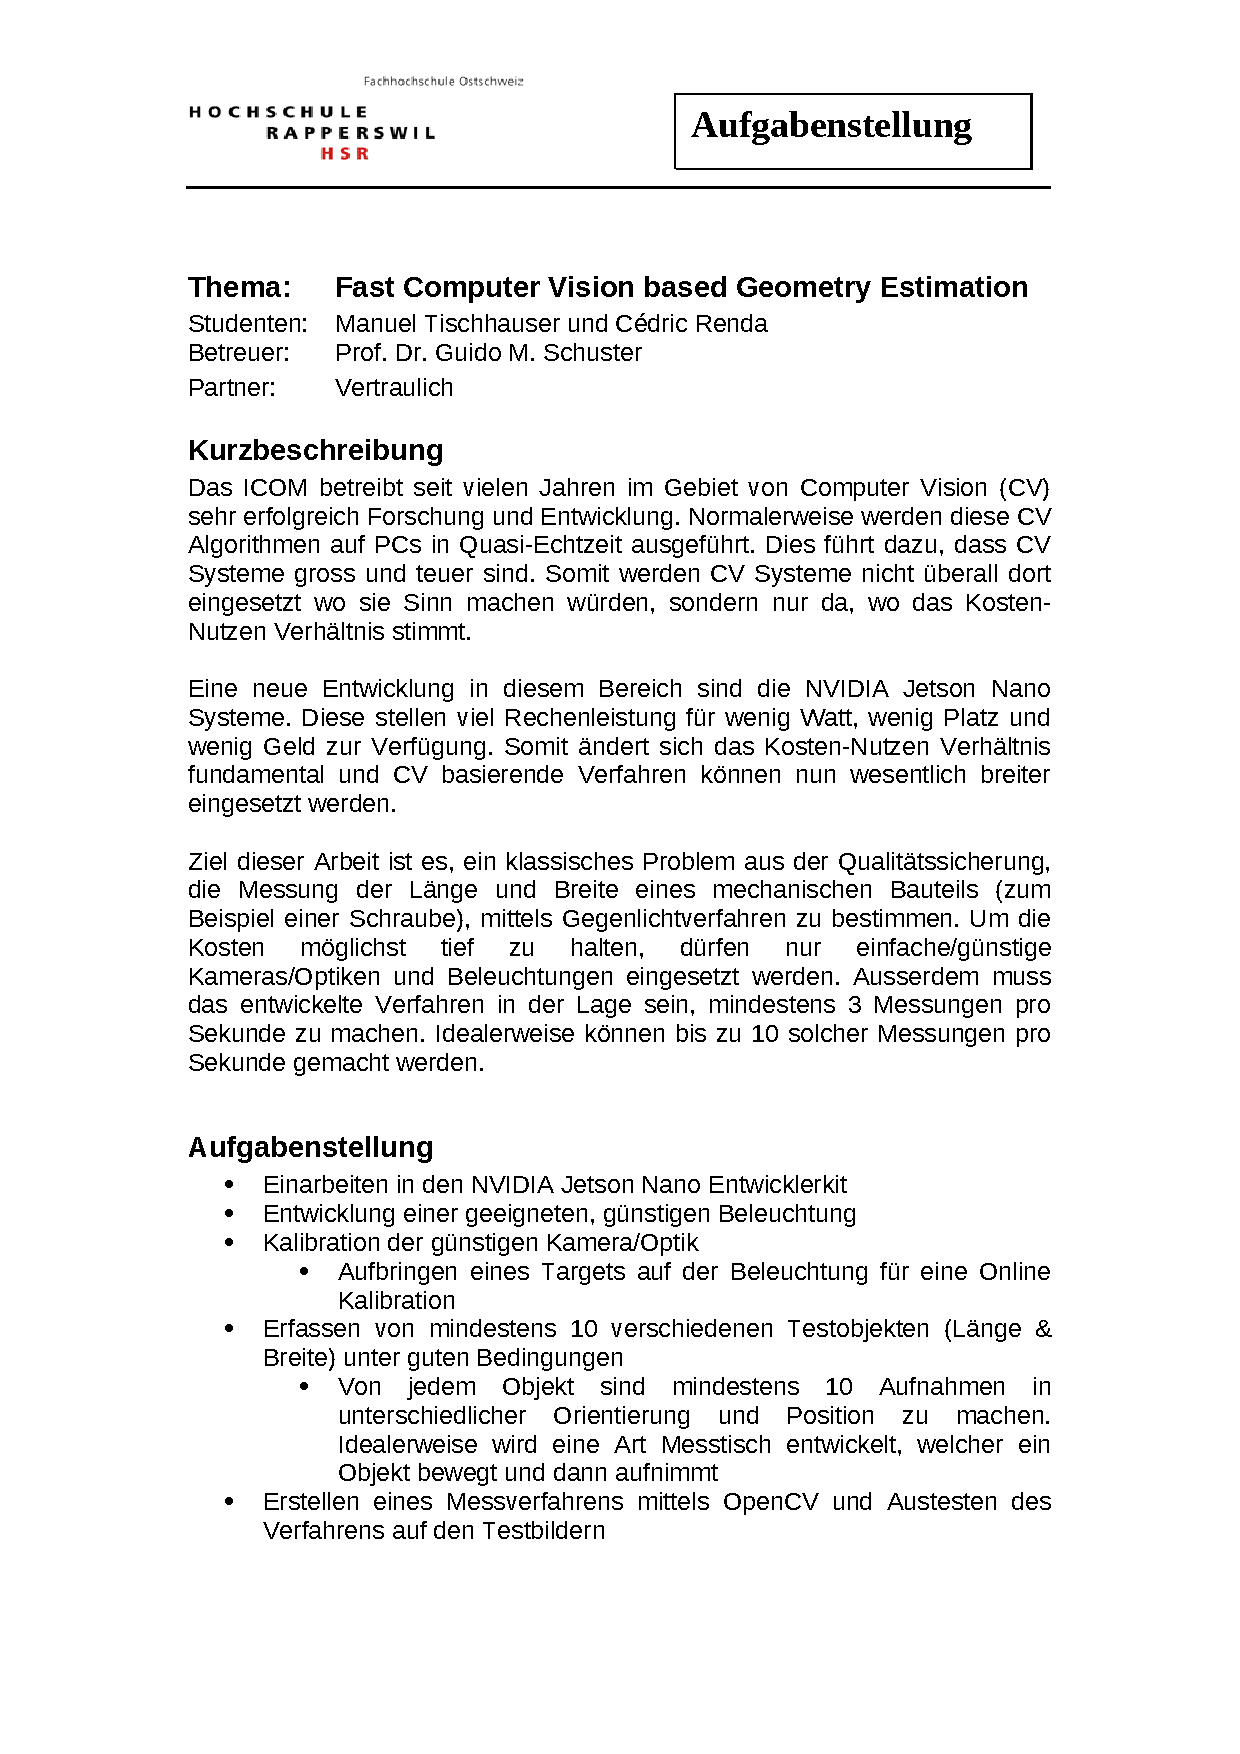
\includegraphics[trim= 0cm 0cm 0cm 0cm,page=1,width=13cm]{FastCVbasedGeometryEstimation.pdf}
\end{figure}
\begin{figure}[H]
	\centering
	\includegraphics[trim= 0cm 0cm 0cm 0cm,page=2,width=13cm]{FastCVbasedGeometryEstimation.pdf}
\end{figure}




\vfill
\pagebreak
\ifodd\value{page}\else\null\clearpage\fi
\lhead{Index}
\rhead{}
\addcontentsline{toc}{chapter}{\indexname}
\input main.ind
\end{document}
